\section{Engineering Background}

\subsection{Testbench Architecture}

% REVISIT: find more testbench architectures to compare with
While there has been many similar performance analysis done on hybrid SoCs
before, each of them uses their own, usually ad hoc, testbench
design~\cite{Shi1}.
This project will use a structure that is inspired by that of an agent in
UVM~\cite{Accellera1}.

\begin{figure}[H]
  \centering
  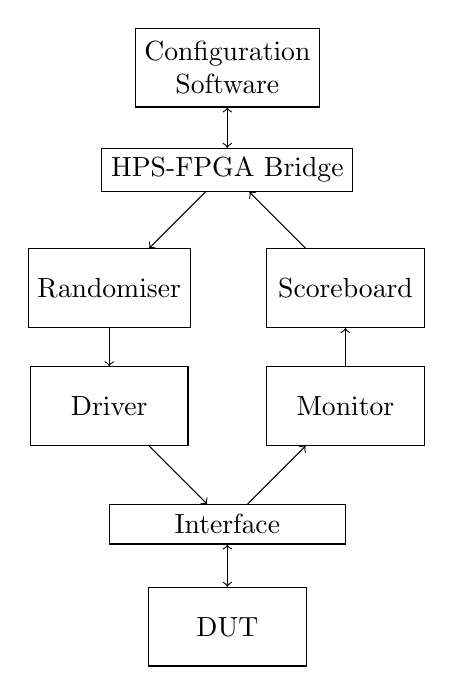
\begin{tikzpicture}
    \tikzset{block/.style= {draw,
                            rectangle,
                            align=center,
                            minimum width=2cm,
                            minimum height=1cm},
             inter/.style= {draw,
                            rectangle,
                            minimum width=3cm,
                            minimum height=0.5cm},
            }
    \path
    (0,3.5)    node[block](r) {Randomiser}
    (0,2)      node[block](d) {Driver}
    (1.5,0.5)  node[inter](i) {Interface}
    (1.5,-0.8) node[block](t) {DUT}
    (3,3.5)    node[block](s) {Scoreboard}
    (3,2)      node[block](m) {Monitor}
    (1.5,5)    node[inter](b) {HPS-FPGA Bridge}
    (1.5,6.3)  node[block](w) {Configuration\\Software}
    ;
    \draw[->]  (r) -- (d);
    \draw[->]  (d) -- (i);
    \draw[<->] (i) -- (t);
    \draw[->]  (i) -- (m);
    \draw[->]  (m) -- (s);
    \draw[->]  (b) -- (r);
    \draw[->]  (s) -- (b);
    \draw[<->] (b) -- (w);
\end{tikzpicture}
  \caption{Proposed testbench block diagram}
  \label{Block}
\end{figure}

Configuration is first done from a software running on the HPS, which sends
the test specifications to the randomiser.
The randomiser will provide a stream of random data, that would be converted
to meaningful test inputs by the driver.
The test output will be watched by the monitor, reporting any interesting
event to the scoreboard, which keeps track of them.
The scoreboard feeds the information back to the software on-demand.
The interface is used to decouple the control logic with the DUT, allowing
the frequency of the DUT to be finely controlled.

\subsection{Target}
The design of the verification system is the major engineering challenge of this
project.
In order to stress the DUT, the verification system must perform at a much
higher frequency than the expected frequency of the DUT.
Assuming the DUT is to run at 300MHz, to fully explore the effect of
overclocking, the testbench must be able to run at double the frequency or
higher.
This gives a target frequency of 800MHz.
Assuming data width of 32-bits, the target data transfer rate is then 
estimated to be 25.6Gbps.

\subsection{Data Transfer Rate}
% REVISIT: possible to find exact bandwidth of the bridge?
As the test is to be controlled on the HPS, the HPS-FPGA bridge will be the
immediate bottleneck if the test data is to flow from HPS to FPGA.
While the HPS can easily generate test data with a piece of software,
there is a large amount of overhead as data crosses from one architecture
to another.
This overhead exists in the form of both a decreased bandwidth and a increased
delay.
Thus, it would not be sensible for the HPS to send out data during runtime.

\subsubsection{\textbf{Off-chip DDR SDRAM}}
Another thought may be to first populate the off-chip DDR SDRAM on FPGA
side, then feed that data to the DUT during test.
This is already much faster than passing the data directly from HPS.
The 1GB, 32-bits wide DDR3 on FPGA side is rated at 400MHz.
With double rate transfer, this gives a maximum transfer rate of 25.6Gbps.

While using the off-chip RAM may theoretically achieve the targets,
it still has its disadvantages.
First, the process of filling up the memory and then using them for the tests
takes time.
This means the test would be broken up into bursts with time in between for
checking results and filling in new data.
The complexity of the SDRAM interface also requires a SDRAM controller to be
used to manage SDRAM refresh cycles, address multiplexing and interface timing.
These all adds up to a significant access latency.
While it could be overcame with burst accesses and piplined accesses,
it would further complicate the SDRAM controller.
A controller is provided by Altera~\cite{Altera3}, but it consumes
a non-negligible amount of the limited FPGA resources, while adding
unnecessary complexities to the design.
Customising or building a new SDRAM controller to fit this project is possible,
but needlessly time-consuming.

\subsubsection{\textbf{On-chip Memory}}
The on-chip memory is much faster and simpler to handle.
In comparison, this memory is implemented on the FPGA itself, and thus needs
no external connections for accesses.
It has the highest possible throughput, with the lowest possible latency
in an FPGA-based system.
The memory transactions can also be piplined, giving one transaction per
clock cycle.
With an on-chip FIFO accessed in dual-port mode, the write operations at one
end and the read operations at the other end can happen simultaneously.
This effective doubling of the bandwidth is useful as tests are prepared
and fed into the DUT, or when test results are collected and fed to the
monitor.

On-chip memory is not without its drawbacks.
It is volatile and very limited in capacity.
While the off-chip can have its storage reaching 1GB, that of the on-chip
memory could only reach a few MB~\cite{Altera2}.
Volatility is not exactly of concern in this project, but its small capacity
means not much test data can be held before it needs more fed in.

\subsection{Runtime Test Data Generation}
To exploit the benefits of on-chip memory, a way of generating test data
at runtime needs to be designed.
As arithmetic operators have a vast set of valid inputs, it is necessary to
have cost effective test generation.

A good choice here is to use random testing.
With relatively minimum effort, random testing can provide significant coverage
and discover relatively subtle errors~\cite{Duran1}.
The main drawback of random testing is the possible lack of coverage on extreme
cases, and the usual solution is to provide handwritten tests to complement
random testing.
However, as the main goal of this testbench is gauging the performance of
the module, and not necessarily verifying the correctness of it,
this could be ignored during stress testing.
If logic correctness testing is later required, these special tests could be
written and run separately with a relaxed timing restriction.

LFSRs are a reliable way of generating pseudo random numbers fast with minimum
cost~\cite{Hazwani1}.
They will thus form the starting point of data generation.
While it is possible for data generated to be invalid as inputs to the DUT, this
should not be the case for most benchmarks in this project.
Even if so, they can be dealt with at the monitor.

With this, the software would only need to configure the randomiser, and test
data no longer needs to pass through the HPS-FPGA bridge.

\subsection{Clock Domains}
Another concern in the system design is of the different clock domains that
must exist on the FPGA.
At a minimum, there needs to be two clock domains, one surrounds the DUT and
another supports the rest of the control logic around the DUT.
These clock frequencies can be generated and distributed with PLLs, which are
provided as IP Cores in the Quartus software~\cite{Altera4}.
Data crossing clock domains will be fed through FIFOs to prevent loss.

The proposed structure will have the main bulk of the control logic running
on a separate clock domain as the DUT.
Only an interface with FIFOs and minimum logic will be running in synchronous
with the DUT.
Therefore, the test controls can be running at a slower frequency without
bottlenecking the system, allowing the DUT to be stressed further.

\subsection{Result Analysis}
If the monitor detects an interesting event such as an error, it will sent out
a message to the scoreboard.
The scoreboard has counters tracking these events, and update them back to the
software periodically.

The software can run statistics to provide further insights to the user.